\documentclass[border=0.2cm]{standalone}
\usepackage{tikz}
\begin{document}


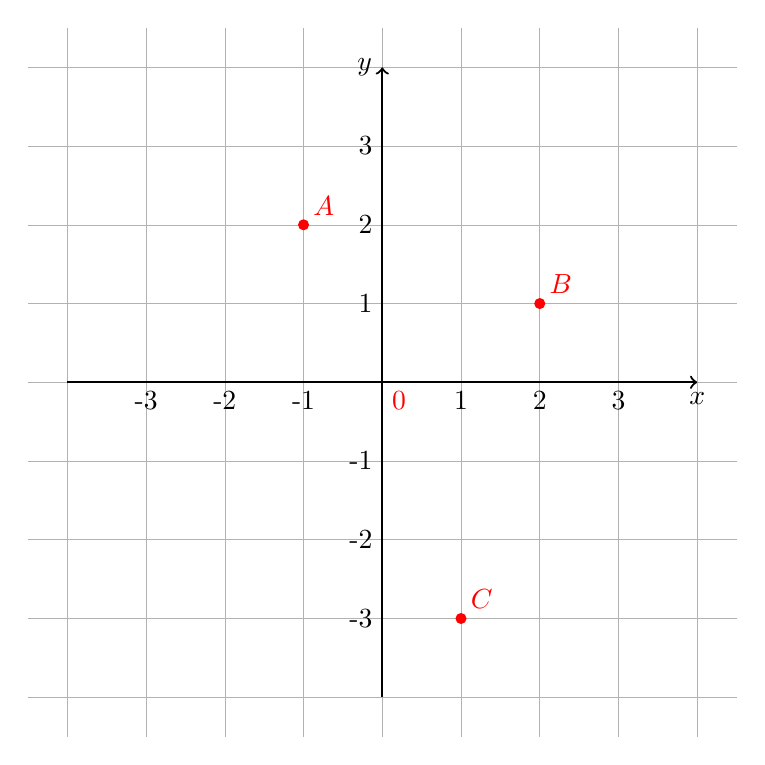
\begin{tikzpicture}
  \draw[help lines,black!30] (-4.5,-4.5) grid (4.5,4.5);
  \draw[thick,->] (0,-4) -- (0,4) node[left]  {$y$};
  \draw[thick,->] (-4,0) -- (4,0) node[below] {$x$};
  \foreach \x in {-3,-2,-1,1,2,3} \node[left] at (0,\x) {\x} node[below] at (\x,0) {\x};
  \node[below right,color=red] at (0,0) {0}; 


  \coordinate (a) at (-1,2);
  \coordinate (b) at (2,1);
  \coordinate (c) at (1,-3);

  \fill[red] (a) circle (2pt) node[above right] {$A$};
  \fill[red] (b) circle (2pt) node[above right] {$B$};
  \fill[red] (c) circle (2pt) node[above right] {$C$};

  \end{tikzpicture}



\end{document}